% ******************************** REQUISITI ********************************
\subsection{Tabella di categorizzazione dei requisiti}
\begin{adjustbox}{width=.8\paperwidth, height=.8\paperheight, center}
	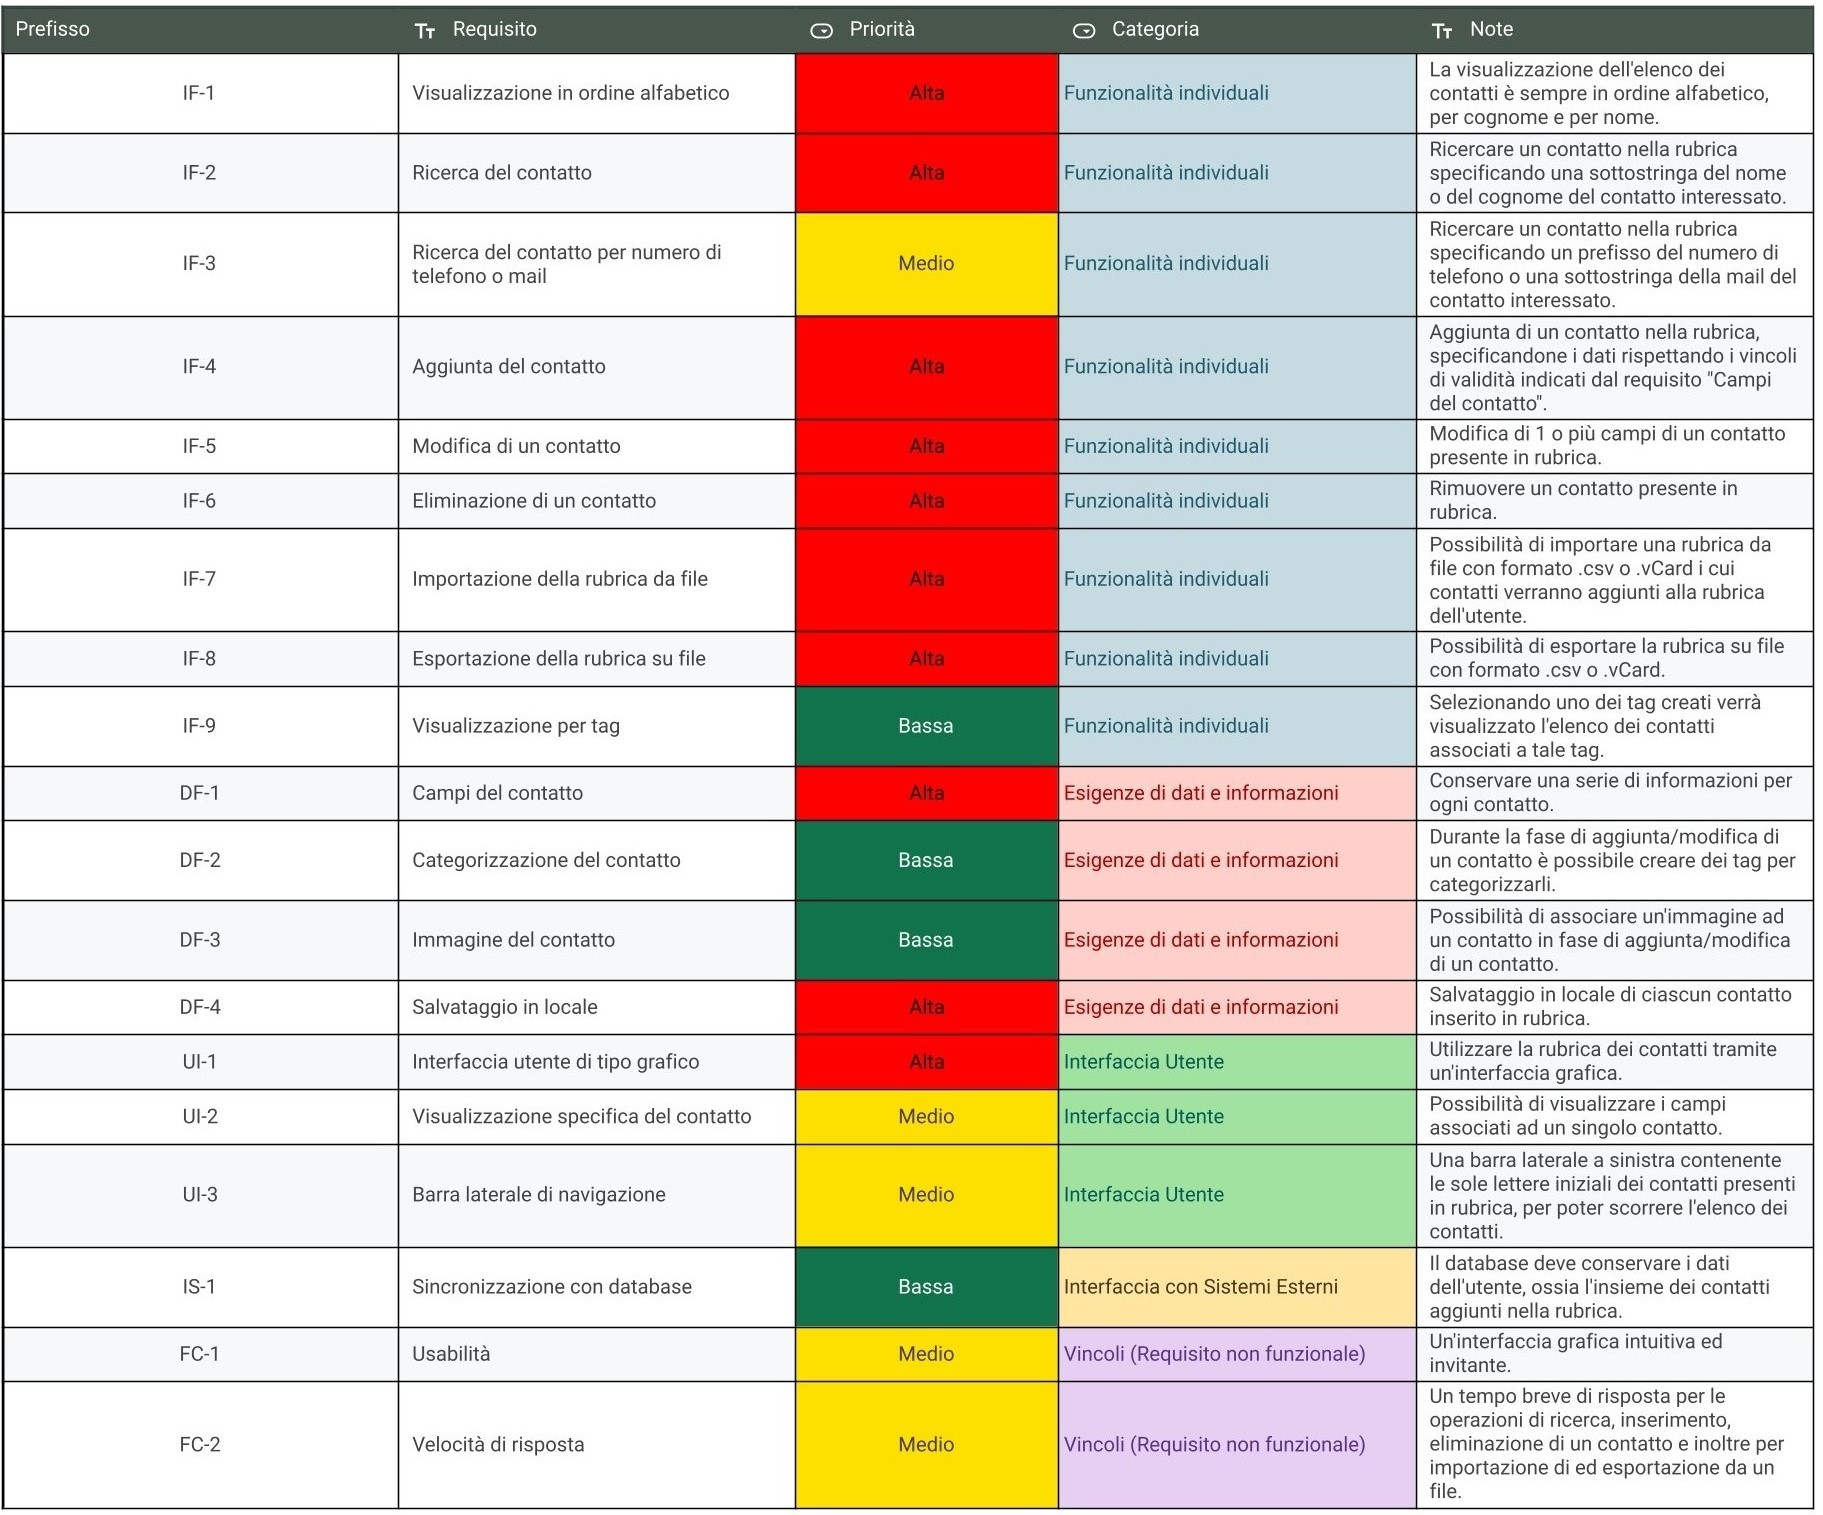
\includegraphics{images/Categorizzazione requisiti.jpg}
\end{adjustbox}
\captionof{figure}{Tabella di categorizzazione dei requisiti}
\label{categorizzazione_dei_requisiti}

\newpage
\subsection{Requisiti Funzionali}
	\begin{tcolorbox}[breakable, colback=white,colframe=black!80!white,title=\textbf{Funzionalità individuali IF}]
	\begin{itemize}[itemsep=2pt, topsep=0pt]
		\hypertarget{IF-1}{\item[\textbf{IF-1}]} \textbf{Visualizzazione in ordine alfabetico}
		\\I contatti sono sempre visualizzati in ordine alfabetico, ordinandoli per cognome e nome. 
		\\Si offre la possibilità di poter scegliere, cliccando sull’icona dell’imbuto 
\includegraphics[height=0.4cm]{images/imbuto_icona.jpeg}, tra l’ordinamento A-Z oppure Z-A rispetto al nome o al cognome.
		\\Anche usufruendo della visualizzazione per Tag l’ordine dei contatti è sempre alfabetico (vedi \hyperlink{IF-9}{IF-9}).
		
		\item[\textbf{IF-2}] \textbf{Ricerca del contatto}
		\\L’utente può cercare il contatto desiderato inserendo nella casella di ricerca una sottostringa del nome o del cognome del contatto desiderato.
		\\Verranno visualizzati, secondo l’ordine alfabetico stabilito in \hyperlink{IF-1}{IF-1}, i contatti che rispettano il requisito di ricerca.
		
		\item[\textbf{IF-3}] \textbf{Ricerca per numero di telefono o mail}
		\\L’utente può cercare il contatto desiderato inserendo nella casella di ricerca un suffisso del numero di telefono o una sottostringa della mail associati al contatto. 
		\\Verranno visualizzati, secondo l’ordine alfabetico stabilito in \hyperlink{IF-1}{IF-1}, i contatti che rispettano il requisito di ricerca.				
		
		\item[\textbf{IF-4}] \textbf{Aggiunta del contatto}
		\\L’utente ha la possibilità di aggiungere un contatto alla sua rubrica.
		\\In particolare cliccando sul simbolo “+” oppure attraverso il menù a tendina “Rubrica”, compare una schermata in cui è possibile inserire i campi del contatto (definiti in \hyperlink{DF-1}{DF-1}, \hyperlink{DF-2}{DF-2}, \hyperlink{DF-3}{DF-3}).
		Successivamente si può salvare il nuovo contatto o annullare l’operazione con i rispettivi pulsanti “Salva” o “Annulla”.
		\\E’ possibile aggiungere un nuovo contatto contenente gli stessi valori dei campi di 1 o più contatti già esistenti.		
		
		\item[\textbf{IF-5}] \textbf{Modifica di un contatto}
		\\L’utente ha la possibilità di modificare un contatto dalla sua rubrica.
		\\Cliccando su un contatto e premendo sul pulsante “Modifica” è possibile modificare i suoi campi (definiti in \hyperlink{DF-1}{DF-1}, \hyperlink{DF-2}{DF-2}, \hyperlink{DF-3}{DF-3}). 
		\\Dopo aver effettuato modifiche è possibile annullare o salvare l’operazione con i pulsanti “Salva” o “Annulla”.
		
		\item[\textbf{IF-6}] \textbf{Eliminazione di un contatto}
		\\L’utente ha la possibilità di eliminare un contatto dalla sua rubrica. 
		\\In particolare cliccando su un contatto e premendo sul pulsante “Elimina”, l’utente potrà confermare o meno l’operazione attraverso una schermata di conferma.
		
		\item[\textbf{IF-7}] \textbf{Importazione della rubrica da file}
		\\L’utente può scegliere, tramite la sezione del menù a tendina “File”, di importare una rubrica con 0 o più contatti da un file \texttt{.csv} o \texttt{.vCard}. 
		\\Gli eventuali contatti presenti nella rubrica importata verranno aggiunti alla rubrica dell’utente. 
		\\L’utente può interrompere l’operazione in qualsiasi momento.
	
		\item[\textbf{IF-8}] \textbf{Esportazione della rubrica su file}
		\\L’utente può scegliere, tramite la sezione del menù a tendina “File”, di esportare la sua rubrica, includendo tutti i contatti oppure quelli associati ad un particolare Tag selezionato da una lista che uscirà al momento dell’esportazione.
		\\L’utente può scegliere di esportare la rubrica in un file \texttt{.csv} o \texttt{.vCard} e specificare il nome del file. 
		
		\hypertarget{IF-9}{\item[\textbf{IF-9}]} \textbf{Visualizzazione per tag}
		\\L’utente cliccando sull’icona dell’imbuto 
\includegraphics[height=0.4cm]{images/imbuto_icona.jpeg} può scegliere 1 o più Tag tra quelli presenti che comporta la visualizzazione dei soli contatti associati al/ai Tag selezionato/i.
		\\La visualizzazione segue i criteri definiti in \hyperlink{IF-1}{IF-1}.		
	\end{itemize}
\end{tcolorbox}

\begin{tcolorbox}[colback=white,colframe=black!80!white,title=\textbf{Esigenze dei dati e informazioni DF}]
	\begin{itemize}[itemsep=2pt, topsep=0pt]
		\hypertarget{DF-1}{\item[\textbf{DF-1}]} \textbf{Campi del contatto}
		\\Per ogni contatto bisogna conservare i seguenti dati:
		\begin{itemize}[noitemsep, topsep=0pt, label=$\bullet$]
			\item cognome e/o nome;
			\item da 0 a 3 numeri di telefono;
			\item da 0 a 3 mail.
		\end{itemize}
		Tali dati possono essere aggiunti in fase di creazione del contatto e modificati in qualsiasi momento.
		
		\hypertarget{DF-2}{\item[\textbf{DF-2}]} \textbf{Categorizzazione contatto}
		\\L’utente può aggiungere facoltativamente un ulteriore campo ossia un Tag. 
		\\In particolare l’utente può inserire da 1 a 3 Tag a piacere (ad esempio preferiti, famiglia, lavoro, …) ad ogni contatto in fase di aggiunta/modifica del contatto.
		\\Un Tag è una particolare proprietà che si può associare ad 1 o più contatti.
		\\Attraverso il menù a tendina “Rubrica”, cliccando su “Gestisci Tag”,  l’utente può visualizzare tutti i Tag inseriti precedentemente, e può aggiungerli, rimuoverli o modificarli. 
		\\Per la visualizzazione dei contatti appartenenti ai Tag vedi \hyperlink{IF-9}{IF-9}.		
		
		\hypertarget{DF-3}{\item[\textbf{DF-3}]} \textbf{Immagine contatto}
		\\Ad ogni contatto è associato un ulteriore campo ossia un’immagine.
		In particolare una sagoma grigia che si vedrà nella visione dettagliata del contatto. 
		\\Ma in fase di aggiunta/modifica di un contatto, l’utente può aggiungere un’immagine personalizzata, la quale può essere selezionata tra quelle suggerite dall’applicazione stessa oppure importata dall’esterno.
		
		\hypertarget{DF-4}{\item[\textbf{DF-4}]} \textbf{Salvataggio in locale}
		\\Salvataggio in locale dei contatti inseriti in rubrica nel file binario \texttt{Data.bin}. Quest’ultimo file offre la possibilità all’utente di conservare i contatti, e i relativi campi (vedi \hyperlink{DF-1}{DF-1}, \hyperlink{DF-2}{DF-2}, \hyperlink{DF-3}{DF-3}), in modo che ogniqualvolta che riapre l’applicazione della rubrica visualizza gli stessi contatti della sessione precedente.
		\\Tale salvataggio dei contatti in locale è quello di default se non viene specificata la preferenza di usare un database (vedi \hyperlink{IS-1}{IS-1}).
		\\Oltre al file \texttt{Data.bin}, viene salvato in locale il file binario \texttt{Config.bin} il quale mantiene le impostazioni dell’applicazione, come ad esempio il link del database se questo viene fornito dall’utente.
		
	\end{itemize}
\end{tcolorbox}

\begin{tcolorbox}[colback=white,colframe=black!80!white,title=\textbf{Interfaccia Utente UI}]
	\begin{itemize}[itemsep=2pt, topsep=0pt]
		\item[\textbf{UI-1}] \textbf{Avere interfaccia utente di tipo grafico} 
		\\Tramite l’utilizzo di JavaFX l’utente interagisce con il programma tramite interfaccia grafica, permettendone un utilizzo facilitato e maggiormente intuitivo.
		
		\item[\textbf{UI-2}] \textbf{Visualizzazione specifica del contatto}
		\\Dopo aver selezionato dalla rubrica un contatto, l’utente vedrà la visualizzazione dettagliata del contatto scelto.
		\\In questa sezione sono visibili i campi definiti in \hyperlink{DF-1}{DF-1}, \hyperlink{DF-2}{DF-2}, \hyperlink{DF-3}{DF-3}.		
	\end{itemize}
\end{tcolorbox}

\begin{tcolorbox}[colback=white,colframe=black!80!white,title=\textbf{Interfacce con sistemi esterni IS}]
	\begin{itemize}[itemsep=2pt, topsep=0pt]
		\hypertarget{IS-1}{\item[\textbf{IS-1}]} \textbf{Sincronizzazione con database}
		\\Cliccando sul menù a tendina "File" e poi su "Configurazione" è possibile esprimere la propria preferenza riguardo la possibilità di salvare la propria rubrica su un database esterno, fornendo il link. 
		\\In questo caso, il salvataggio dati non avverrà più in locale, come avviene di default tramite file \texttt{Data.bin} (vedi \hyperlink{DF-4}{DF-4}), ma sul database.
	\end{itemize}
\end{tcolorbox}


\subsection{Requisiti Non Funzionali}
Il software non prevede requisiti non funzionali


% ******************************** CASI D'USO ********************************
\newpage
\subsection{Diagramma dei Casi d'Uso}
\begin{figure}[h]
	\centering
	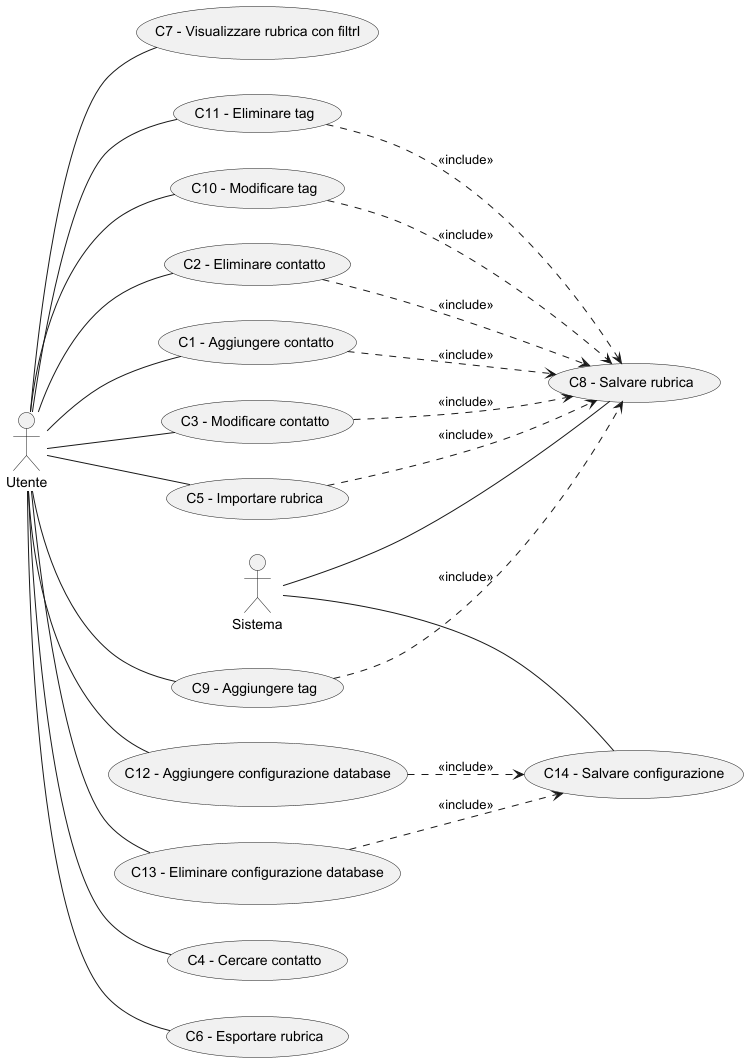
\includegraphics[width=.77\linewidth]{images/DiagrammaCasiD.png}
	\caption{Diagramma UML dei Casi d'uso}
	\label{diagramma_casi_duso1}	
\end{figure}

\newpage
\subsection{Casi d'Uso formato testuale}
\begin{tcolorbox}[colback=white,colframe=black!80!white,title=\textbf{C1 - Aggiungere contatto}]
\textbf{Attore partecipante}: Utente
\\\textbf{Precondizioni}: Utente ha la schermata della rubrica aperta.
\\\textbf{Postcondizioni}: Nella rubrica viene aggiunto un contatto.
\\\textbf{Flusso di eventi normale}:
\begin{enumerate}[noitemsep, topsep=0pt]
\item Utente clicca il pulsante “+”;
\item Utente inserisce il nome e/o il cognome;
\item Utente inserisce da 0 a 3 numeri di telefono;
\item 	Utente inserisce da 0 a 3 mail ;
\item 	Utente inserisce da 0 a 3 Tag;
\item 	Utente inserisce un’immagine;
\item 	Utente salva l’operazione;
\end{enumerate}
\textbf{Flusso di eventi alternativo}:
\begin{itemize}[noitemsep, topsep=0pt]
	\item[1a. ] Utente clicca il menù a tendina “Rubrica”;
	\item[1a.1] Utente crea il contatto;
	\item[6a. ] Utente non inserisce alcuna immagine, quindi rimane quella di default;
	\item[7a. ] Utente annulla l’operazione;
	\item[7a.1] L’esecuzione riprende dal passo 1;
\end{itemize}
\end{tcolorbox}

\begin{tcolorbox}[colback=white,colframe=black!80!white,title=\textbf{C2 - Eliminare contatto}]
	\textbf{Attore partecipante}: Utente
	\\\textbf{Precondizioni}: Esiste almeno un contatto nella rubrica.
	\\\textbf{Postcondizioni}: Viene rimosso dalla rubrica il contatto selezionato.
	\\\textbf{Flusso di eventi normale}:
	\begin{enumerate}[noitemsep, topsep=0pt]
\item	Utente seleziona il contatto da eliminare;
\item	Utente clicca il pulsante “Elimina”;
\item	Utente conferma l’operazione dalla schermata di conferma;
	\end{enumerate}
	\textbf{Flusso di eventi alternativo}:
	\begin{itemize}[noitemsep, topsep=0pt]
		\item[3a. ] Utente annulla l’operazione dalla schermata di conferma;
		\item[3a.1] L’esecuzione riprende dal passo 1;
	\end{itemize}
\end{tcolorbox}

\begin{tcolorbox}[colback=white,colframe=black!80!white,title=\textbf{C3 - Modificare contatto}]
	\textbf{Attore partecipante}: Utente
	\\\textbf{Precondizioni}: Esiste almeno un contatto nella rubrica.
	\\\textbf{Postcondizioni}: Viene modificato il contatto selezionato.
	\\\textbf{Flusso di eventi normale}:
	\begin{enumerate}[noitemsep, topsep=0pt]
\item Utente seleziona il contatto da modificare;
\item Utente clicca il pulsante “Modifica”; 
\item Utente modifica uno o più campi del contatto;
\item Utente salva l’operazione;	
	\end{enumerate}
	\textbf{Flusso di eventi alternativo}:
	\begin{itemize}[noitemsep, topsep=0pt]
		\item[4a. ] Utente annulla l’operazione;
		\item[4a.1] L’esecuzione riprende dal passo 1;
	\end{itemize}
\end{tcolorbox}

\begin{tcolorbox}[colback=white,colframe=black!80!white,title=\textbf{C4 - Cercare contatto}]
	\textbf{Attore partecipante}: Utente
	\\\textbf{Precondizioni}: Utente ha la schermata della rubrica aperta.
	\\\textbf{Postcondizioni}: I contatti che rispettano il criterio di ricerca vengono visualizzati.
	\\\textbf{Flusso di eventi normale}:
	\begin{enumerate}[noitemsep, topsep=0pt]
		\item Utente scrive nella casella di ricerca una sottostringa del nome o del cognome del contatto da cercare;
	\end{enumerate}
	\textbf{Flusso di eventi alternativo}:
	\begin{itemize}[noitemsep, topsep=0pt]
		\item[1a.] Utente scrive nella casella di ricerca un prefisso del numero di tel. del contatto da cercare;
		\item[1b.] Utente scrive nella casella di ricerca una sottostringa della mail del contatto da cercare;
	\end{itemize}
\end{tcolorbox}

\begin{tcolorbox}[colback=white,colframe=black!80!white,title=\textbf{C5 - Importare rubrica}]
	\textbf{Attore partecipante}: Utente
	\\\textbf{Precondizioni}: Utente possiede un file \texttt{.csv} o \texttt{.vCard}
	\\\textbf{Postcondizioni}: Vengono caricati nella rubrica dell’utente i contatti contenuti nel file fornito.
	\\\textbf{Flusso di eventi normale}:
	\begin{enumerate}[noitemsep, topsep=0pt]
		\item Utente clicca il menù a tendina “File”;
		\item Utente clicca il pulsante “Importa”;
		\item Utente fornisce il file con estensione \texttt{.csv} o \texttt{.vCard};
		\item Utente seleziona il file;
		\item Utente importa il file;	
	\end{enumerate}
	\textbf{Flusso di eventi alternativo}:
	\begin{itemize}[noitemsep, topsep=0pt]
		\item[3a. ] Utente annulla l’operazione;
		\item[3a.1] L’esecuzione riprende dal passo 1;
		\item[4a. ] Utente fornisce un file con contenuto non interpretabile dalla rubrica;
		\item[4a.1] L’esecuzione riprende dal passo 3;
		\item[5a. ] Utente annulla l’operazione;
		\item[5a.1] L’esecuzione riprende dal passo 1;
		
	\end{itemize}
\end{tcolorbox}

\begin{tcolorbox}[colback=white,colframe=black!80!white,title=\textbf{C6 - Esportare rubrica}]
	\textbf{Attore partecipante}: Utente
	\\\textbf{Precondizioni}: Utente ha la schermata della rubrica aperta.
	\\\textbf{Postcondizioni}: Viene prodotto un file \texttt{.csv} o \texttt{.vCard} con i contatti selezionati.
	\\\textbf{Flusso di eventi normale}:
	\begin{enumerate}[noitemsep, topsep=0pt]
		\item Utente clicca il menù a tendina “File”;
		\item Utente clicca il pulsante “Esporta”;
		\item Utente sceglie la categoria dei contatti da esportare
		\item Utente sceglie l’estensione del file tra l’opzione \texttt{.csv} e \texttt{.vCard};
		\item Utente sceglie il percorso dove salvare il file;
		\item Utente salva l’operazione;	
	\end{enumerate}
	\textbf{Flusso di eventi alternativo}:
	\begin{itemize}[noitemsep, topsep=0pt]
		\item[3a. ] Utente annulla l’operazione;
		\item[3a.1] L’esecuzione riprende al passo 1;
		\item[4a. ] Utente annulla l’operazione;
		\item[4a.1] L’esecuzione riprende al passo 1;
		\item[5a. ] Utente annulla l’operazione;
		\item[5a.1] L’esecuzione riprende al passo 1;
		\item[6a. ] Utente annulla l’operazione;
		\item[6a.1] L’esecuzione riprende al passo 1;	
	\end{itemize}
\end{tcolorbox}

\begin{tcolorbox}[colback=white,colframe=black!80!white,title=\textbf{C7 - Visualizzare rubrica con filtri}]
	\textbf{Attore partecipante}: Utente
	\\\textbf{Precondizioni}: Utente ha la schermata della rubrica aperta.
	\\\textbf{Postcondizioni}: Utente visualizza i contatti associati al filtro selezionato.
	\\\textbf{Flusso di eventi normale}:
	\begin{enumerate}[noitemsep, topsep=0pt]
		\item Utente clicca il pulsante dell’imbuto 
\includegraphics[height=0.4cm]{images/imbuto_icona.jpeg};
		\item Utente sceglie 1 o più Tag tra quelli presenti.
	\end{enumerate}
	\textbf{Flusso di eventi alternativo}:
	\begin{itemize}[noitemsep, topsep=0pt]
		\item[2a.] Utente sceglie l’ordine alfabetico inverso.
		\item[2b.] Utente sceglie l’ordine per nome.
	\end{itemize}
\end{tcolorbox}

\begin{tcolorbox}[colback=white,colframe=black!80!white,title=\textbf{C8 - Salvare rubrica}]
	\textbf{Attore partecipante}: Sistema
	\\\textbf{Precondizioni}: Utente ha effettuato una qualsiasi modifica (aggiunge contatto, elimina Tag, importa un file di una rubrica, …). 
	\\\textbf{Postcondizioni}: Il Sistema salva la modifica.
	\\\textbf{Flusso di eventi normale}:
	\begin{enumerate}[noitemsep, topsep=0pt]
		\item La modifica viene salvata in locale nel file binario \texttt{Data.bin}.
	\end{enumerate}
	\textbf{Flusso di eventi alternativo}:
	\begin{itemize}[noitemsep, topsep=0pt]
		\item[1a.] La modifica viene salvata sul database.
	\end{itemize}
\end{tcolorbox}

\begin{tcolorbox}[colback=white,colframe=black!80!white,title=\textbf{C9 - Aggiungere Tag}]
	\textbf{Attore partecipante}: Utente
	\\\textbf{Precondizioni}: Utente ha la schermata della rubrica aperta.
	\\\textbf{Postcondizioni}: 1 Tag è stato aggiunto.
	\\\textbf{Flusso di eventi normale}:
	\begin{enumerate}[noitemsep, topsep=0pt]
		\item Utente clicca il menù a tendina “Rubrica”;
	\item	Utente clicca il pulsante “Gestisci Tag”;
	\item	Utente aggiunge un nuovo Tag;
	\item	Utente salva l’operazione.		
	\end{enumerate}
	\textbf{Flusso di eventi alternativo}:
	\begin{itemize}[noitemsep, topsep=0pt]
		\item[4a. ] Utente annulla l’operazione;
		\item[4a.1] L’esecuzione riprende al passo 1;		
	\end{itemize}
\end{tcolorbox}

\begin{tcolorbox}[colback=white,colframe=black!80!white,title=\textbf{C10 - Modificare Tag}]
	\textbf{Attore partecipante}: Utente
	\\\textbf{Precondizioni}: Utente ha la schermata della rubrica aperta. 
	\\\textbf{Postcondizioni}: 1 Tag è stato modificato.
	\\\textbf{Flusso di eventi normale}:
	\begin{enumerate}[noitemsep, topsep=0pt]
		\item Utente clicca il menù a tendina “Rubrica”;
		\item Utente clicca il pulsante “Gestisci Tag”;
	\item 	Utente modifica un Tag precedentemente aggiunto;
	\item 	Utente salva l’operazione.		
	\end{enumerate}
	\textbf{Flusso di eventi alternativo}:
	\begin{itemize}[noitemsep, topsep=0pt]
		\item[4a. ] Utente annulla l’operazione;
		\item[4a.1] L’esecuzione riprende al passo 1;		
	\end{itemize}
\end{tcolorbox}

\begin{tcolorbox}[colback=white,colframe=black!80!white,title=\textbf{C11 - Eliminare Tag}]
	\textbf{Attore partecipante}: Utente
	\\\textbf{Precondizioni}: Utente ha la schermata della rubrica aperta.
	\\\textbf{Postcondizioni}: 1 Tag è stato eliminato.
	\\\textbf{Flusso di eventi normale}:
	\begin{enumerate}[noitemsep, topsep=0pt]
		\item Utente clicca il menù a tendina “Rubrica”;
	\item	Utente clicca il pulsante “Gestisci Tag”;
	\item	Utente seleziona il Tag che vuole eliminare;
	\item	Utente conferma l’operazione dalla schermata di conferma;
	\end{enumerate}
	\textbf{Flusso di eventi alternativo}:
	\begin{itemize}[noitemsep, topsep=0pt]
		\item[4a. ] Utente annulla l’operazione dalla schermata di conferma;
		\item[4a.1] L’esecuzione riprende dal passo 1;		
	\end{itemize}
\end{tcolorbox}

\begin{tcolorbox}[colback=white,colframe=black!80!white,title=\textbf{C12 - Aggiungere configurazione database}]
	\textbf{Attore partecipante}: Utente
	\\\textbf{Precondizioni}: Utente ha la schermata della rubrica aperta.
	\\\textbf{Postcondizioni}: Utente ha aggiunto il link del database.
	\\\textbf{Flusso di eventi normale}:
	\begin{enumerate}[noitemsep, topsep=0pt]
		\item Utente clicca il menù a tendina “File”;
		\item Utente clicca il pulsante “Configurazione”;
		\item Utente fornisce il link del database scelto.		
	\end{enumerate}
	\textbf{Flusso di eventi alternativo}:
	\begin{itemize}[noitemsep, topsep=0pt]
		\item[3a. ] Utente aggiunge un link non valido;
		\item[3a.1] L’esecuzione riprende al passo 3;
	\end{itemize}
\end{tcolorbox}

\begin{tcolorbox}[colback=white,colframe=black!80!white,title=\textbf{C13 - Eliminare configurazione database}]
	\textbf{Attore partecipante}: Utente
	\\\textbf{Precondizioni}: Utente ha inserito precedentemente il link del database.
	\\\textbf{Postcondizioni}: Utente ha eliminato il link del database.
	\\\textbf{Flusso di eventi normale}:
	\begin{enumerate}[noitemsep, topsep=0pt]
		\item Utente clicca il menù a tendina “File”;
		\item Utente clicca il pulsante “Configurazione”;
		\item L’utente sceglie di rimuovere il link del database;
		\item Utente conferma l’operazione dalla schermata di conferma.
	\end{enumerate}
	\textbf{Flusso di eventi alternativo}:
	\begin{itemize}[noitemsep, topsep=0pt]
		\item[3a. ] Utente annulla l’operazione dalla schermata di conferma;
		\item[3a.1]	L’esecuzione riprende dal passo 3.
	\end{itemize}
\end{tcolorbox}

\begin{tcolorbox}[colback=white,colframe=black!80!white,title=\textbf{C14 - Salvare configurazione}]
	\textbf{Attore partecipante}: Sistema
	\\\textbf{Precondizioni}: Utente ha modificato le configurazioni dell’applicazione (ad esempio aggiunta o eliminazione del link del database)
	\\\textbf{Postcondizioni}: Il sistema salva la modifica.
	\\\textbf{Flusso di eventi normale}:
	\begin{enumerate}[noitemsep, topsep=0pt]
		\item Sistema salva la modifica in locale in un file di configurazione \texttt{Config.bin}.
	\end{enumerate}
	\textbf{Flusso di eventi alternativo}: /
\end{tcolorbox}
